
\chapter{Stability of equilibrium points and bifurcations}

\begin{center}
\colorbox{LightBlue}{\parbox{1\textwidth}{\noindent{\bf Note:} There is no need to repeat the information provided during the guided session. Answer the questions as concise and accurate as possible. Use graphical and/or tabular presentation rather than full sentences. The \textit{page limit} 
for this exercise is \textit{4 printed pages}, including figures.}}
\end{center}

% \section{Bead on a tilted wire}

% A bead with mass $m$ moves along a wire, tilted with angle
% $\theta$. A spring with length $L_0$ in relaxed state and with
% spring constant $k$, is fixed to the bead. The motion of the bead
% is damped by a friction force $b\dot{x}$. The construction is
% shown in the following figure.

% \begin{center}
%     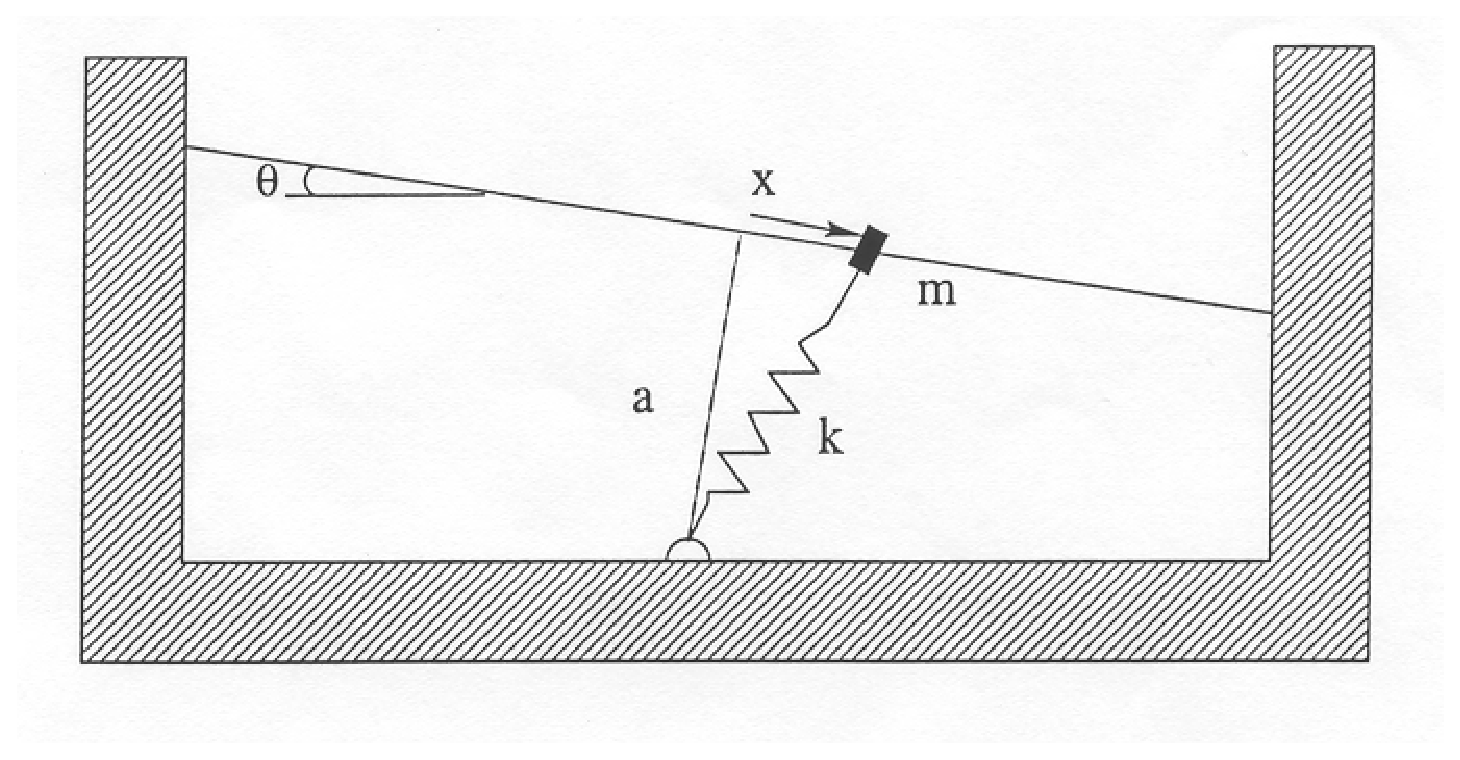
\includegraphics[scale=0.4]{bead}
%     %width=480pt,height=600pt
% \end{center}

% \subsection{System model}

% Given the system model of the bead on a tilted wire
% \begin{equation*}
% m\frac{d^2x}{dt^2}=mg\sin\theta -b\frac{dx}{dt}-kx\left(1-\frac{L_0}{\sqrt{x^2+a^2}}\right).
% \end{equation*}

% \subsection{The case $\theta=0$}

% \begin{enumerate}

% \item Give all fixed points in terms of $k, a, m, b$ and $L_0$.

% \item What is their stability in the case that also $m=0$? Draw a bifurcation diagram for a suitable
% free parameter.

% \item For which relative value of $m$ (different from 0) can the inertia term be neglected and the system be reduced to a first order system? \\
% \textbf{Hint:} make the system dimensionless by dividing by $ak$.

% \item Show that the original differential equation can be transformed to
% \begin{eqnarray*}
% \frac{\partial u}{\partial \tau} & = & v \\
% \frac{\partial v}{\partial \tau} & = & - \frac{1}{\epsilon} [v + (1- \frac{R}{\sqrt{1+u^2}}) u ] \\
% \end{eqnarray*}
% and compare the behaviour via simulation with the behaviour of the
% first order system
% \[ \frac{\partial u}{\partial \tau} = - (1- \frac{R}{\sqrt{1+u^2}}) u \]
% for a fixed $R<1$ (R value depends on your group) and several
% values of $\epsilon$.  To this end, you can use Matlab's
% \verb!ode45! solver.

% \end{enumerate}

% \subsection{The case $\theta \neq 0$}

% \begin{enumerate}

% \item Show that the equilibrium equation can be rewritten in dimensionless form as :
% \[ 1 - \frac{h}{u} = \frac{R}{\sqrt{1+u^2}}\]
% when making an appropriate choice for $R, h$ and $u$.

% \item Give a graphical analysis of the dimensionless equilibrium equation for the cases $R>1$ and $R<1$. How many fixed points can exist in each case?

% \item Show that the equilibrium equation for $r=R-1$ can be reduced to
% \[ - \frac{1}{2}u^3 +ru + h \simeq 0 \]
% when $r, h$ and $u$ are small. Find an approximating formula for the saddle node bifurcation curves in this limiting case.

% \item Show that the exact equations for the saddle node bifurcation curves can be written in following parametric form:
% \[  h(u) = -u^3 \ \ \ \ \ R(u)=(1+u^2)^{\frac{3}{2}}  \]
% when $-\infty < u < \infty$. Give an accurate plot of the bifurcation curves in the $(r,h)$-plane.

% \item Interpret the results physically, in terms of the original variables.

% \end{enumerate}

% https://www.opendatanetwork.com/entity/310M200US16740/Charlotte_Metro_Area_NC_SC/demographics.population.count?year=2016

\begin{Exercise}[name=A simple population model]\label{EX11}


\pj{The population of Belgium could be modeled as
\begin{equation*}
\dot{N} = \alpha \dfrac{(K-N)}{K}N - \beta N,
\end{equation*}
where $N$ is the number of inhabitants, $K$ is the carrying capacity, $\alpha>0$ is the per capita growth rate, and $\beta>0$ is the per capita mortality rate.}

\Question Study the equilibrium points and their stability as a function of $\alpha$ and $\beta$. Summarize your conclusions by using a table. \pj{Which type of bifurcation occurs?} \rema{Answer with a table and/or figures.} 
\Question Based on data from Eurostat\footnote{\url{https://ec.europa.eu/eurostat/web/population-demography-migration-projections/data/database}}, we can estimate a growth rate of $\alpha=1.09\%$ and a mortality rate of $\beta=0.97\%$ in 2016\footnote{$118\,319$ births and $109\,666$ deaths, neglecting emigration, immigration, acquisition or loss of nationality. The total population was 11 311 117.}. Assume the carrying capacity to be $K=15.3$ million. In 2016, the number of inhabitants was $11\,311\,117$. Describe qualitatively what will happen with the population as $t\rightarrow\infty$, according to this model.

%Consider the system for a non-negative real variable $x$ given by:
%
%\begin{equation*}
%\dot{x} = \alpha x (1- \frac{x}{N})-\beta x,
%\end{equation*}
%
%\noindent
%Where $N > 0, \alpha \geq 0$ and $\beta \geq 0$. The growth of $x$ is logistic and the degradation is linear. Study the equilibrium points and their stability as a function of $\alpha$ and $\beta$. Summarize your conclusions by using a table. Identify the type of bifurcation encountered. 
\end{Exercise}

\newpage

\begin{Exercise}[name=Gene control model]\label{EX12}

Consider the coupled system describing the time evolution of non-negative real number numbers $x$ and $y$ given by:
\begin{equation*}
\left\{
    \begin{aligned}
\dot{x} &= \frac{\alpha_1}{1+ y^r} - x, \\
\dot{y} &= \frac{\alpha_2}{1+ x^r} - y,
\end{aligned}
\right.
\end{equation*}


\noindent
where $\alpha_1 \geq 0$, $\alpha_2 \geq 0$ and $r \geq 0$. This model could describe protein abundances of genes. The first term on the right hand side of the equations represents a repression, the second term \pj{represents} a degradation. 

%\begin{enumerate}
    \Question For \pj{a \emph{repression rate}} $r=0$, find a\pj{nd} classify the fixed points. 
    \Question Consider the special case $\alpha_1 = \alpha_2 = 2$ and $r\pj{>0}$.% \in \mathbb{R}^{+} $. 
    \begin{tasks}%[label=(\alph*)]
        \task \label{task121}Find an obvious equilibrium point and verify numerically \pj{(e.g., using \lstinline{PPLANE})} that it is the only one for $0 \leq r \leq 2$.
        \task \label{task122}Study the stability of this equilibrium analytically. \rema{Report your results in a table and/or some figures.}
        \task \label{task123}\pj{At which value of the repression rate $r$ do you expect a bifurcation? Identify its type.} %By studying the stability as $r \in \mathbb{R}^{+} $ varies, explain at which value you expect a bifurcation and identify the type. 
        Do you think this kind of bifurcation is likely based on the properties of the system? Verify numerically for some values of $r$.
        \task Draw numerically all the qualitatively different phase portraits in the region of interest that occur as the parameter $r$ is varied. \pj{Sketch} the bifurcation diagram using the information of \ref{task121}, \ref{task122} and \ref{task123}.
    \end{tasks}
%\end{enumerate}

\end{Exercise}